% =====================================================================
%  CSE-402 Numerical Analysis, Simulation & Modeling -- Section A
%  Order, cost and stability in diffusion sampling
%
%  Build:  latexmk -pdf main.tex        (or: make)
%  Figures are read from ../figures/ -- run ../run_all.sh to regenerate.
% =====================================================================
\documentclass[11pt,a4paper]{article}

\usepackage[T1]{fontenc}
\usepackage[utf8]{inputenc}
\usepackage{lmodern}
\usepackage[margin=2.4cm]{geometry}
\usepackage{amsmath,amssymb}
\usepackage{booktabs}
\usepackage{graphicx}
\usepackage{caption}
\usepackage{subcaption}
\usepackage{xcolor}
\usepackage{tikz}
\usepackage{pgfplots}
\usepackage{siunitx}
\usepackage[hidelinks]{hyperref}
\usepackage{microtype}

\pgfplotsset{compat=1.18}
\usetikzlibrary{arrows.meta,positioning,calc,fit,backgrounds,decorations.pathreplacing,patterns}

\graphicspath{{../figures/}}

\definecolor{armA}{HTML}{1F6F8B}
\definecolor{armB}{HTML}{C7621F}
\definecolor{armC}{HTML}{3F6B34}
\definecolor{warn}{HTML}{8C3A12}
\definecolor{ink}{HTML}{16283A}
\definecolor{soft}{HTML}{5A6B78}

\sisetup{table-format=1.3, round-mode=places, round-precision=3}

\newcommand{\NFE}{\textsc{nfe}}
\newcommand{\eps}{\varepsilon}
\newcommand{\lam}{\lambda}

\title{\textbf{Order, cost and stability in diffusion sampling}\\[2pt]
\large A numerical-analysis audit of DPM-Solver across three tiers of testbed}
\author{CSE-402 Numerical Analysis, Simulation \& Modeling --- Section A}
\date{}

\begin{document}
\maketitle

\begin{abstract}
\noindent
Diffusion image sampling is an initial-value problem: one integrates the
probability-flow ODE from noise to data, paying one neural-network evaluation
(\NFE) per stage. Lu et al.\ (\emph{DPM-Solver}, NeurIPS 2022) accelerate this by
solving the linear half of the ODE exactly, and validate the result with FID --- an
image-quality score. We instead grade the same solvers by the standards of
numerical analysis: measured convergence order, stability at the stiff boundary
$t\!\to\!0$, and error per \NFE. To make error measurable we build three
testbeds of decreasing reference exactness --- an anisotropic Gaussian with a
closed-form trajectory, a Gaussian/point mixture referenced against
\textsc{dop853}, and the real CIFAR-10 DDPM UNet referenced against a fine grid of
itself --- and three solver arms that separate DPM-Solver's two independent
ideas.

Our central result concerns \emph{Assumption B.1}, the smoothness hypothesis the
paper's order theorem rests on. On the two analytic testbeds, which satisfy it
exactly, every solver in every arm attains its textbook order to within
$0.094$. On the real network, which has no obligation to satisfy it, order
collapses --- and collapses \emph{in proportion to the order claimed}: RK4 falls
from $3.94$ to $1.21$, while explicit Euler falls only from $1.01$ to $0.84$.
Two further findings: the $\lam$-reparameterisation, worth almost nothing on the
exact-score tiers, is worth an order of magnitude on the real network; and the
paper's own \S4.2 instability claim does not reproduce on our stiff Tier-1
problem, for a reason we identify. We report the predictions we got wrong
alongside those we got right.
\end{abstract}

% =====================================================================
\section{The problem, in numerical terms}
% =====================================================================

A diffusion model generates an image by starting from Gaussian noise and
following a deterministic flow to the data manifold. That flow is the
\emph{probability-flow ODE}, and evaluating its right-hand side requires one
forward pass of a large neural network. The network call is essentially the
entire cost of sampling, so the governing question is how few evaluations one
can afford before the trajectory leaves the manifold. The unit of cost is the
\NFE, the number of function evaluations.

The base paper's contribution is a change of variables. The right-hand side
splits into a linear part, which is exactly integrable in closed form, and a
neural part, which is not. Classical explicit schemes approximate both at once
and waste error budget on the half that was free. DPM-Solver treats the linear
half exactly and spends its entire approximation on the hard half, reaching good
samples in 10--20 \NFE\ where prior samplers needed 100--250.

The paper proves an order theorem for this scheme and validates it with FID
scores on generated images. FID is a distributional measure of image quality; it
is not a measure of how accurately an ODE was integrated. Three quantities a
numerical analyst would ask for are absent:

\begin{description}
\item[Order.] Halving the step size $h$ should reduce the error by $2^{p}$ for a
$p$th-order method. Nobody measured $p$ against a known-correct trajectory.
\item[Stability.] The ODE stiffens as $t\!\to\!0$ because $\sigma(t)\!\to\!0$.
\S4.2 of the paper \emph{asserts} that classical explicit methods destabilise
there and cites the literature; it never measures a stability limit.
\item[Cost.] A higher-order method is more accurate per step but calls the
network more times per step. Whether it wins after dividing out is an empirical
question.
\end{description}

This report supplies all three, and in doing so tests a hypothesis the paper
states but does not check.

% =====================================================================
\section{Mathematical setting}
% =====================================================================

We use the variance-preserving linear schedule of the base paper, with
$\beta_0 = 0.1$, $\beta_1 = 20$, and $t$ running from $T=1$ down to a small
$t_{\text{end}}$:
\begin{align}
\log \alpha(t) &= -\tfrac{\beta_1-\beta_0}{4}t^2 - \tfrac{\beta_0}{2}t,
&\sigma(t) &= \sqrt{1-\alpha(t)^2}, \\
\beta(t) &= \beta_0 + t(\beta_1-\beta_0),
&f(t) &= \tfrac{\mathrm{d}\log\alpha}{\mathrm{d}t} = -\tfrac{1}{2}\beta(t),
\qquad g^2(t) = \beta(t).
\end{align}

The half log-SNR $\lam(t) = \log\alpha(t) - \log\sigma(t)$ is the natural time
variable for this problem. It is \emph{strictly decreasing} in $t$: $t=1$ gives
the most negative $\lam$, and $t\!\to\!0$ sends $\lam\!\to\!+\infty$. Its inverse
has a cancellation-free closed form,
\begin{equation}
t(\lam) = \frac{2u}{\sqrt{\beta_0^2 + 2(\beta_1-\beta_0)u} + \beta_0},
\qquad u = \log\!\left(e^{-2\lam}+1\right).
\end{equation}

Writing $\eps(x,t)$ for the noise-prediction model --- a network in general, an
exact formula on our analytic tiers --- the same trajectory admits three
discretisable forms, and these define our three solver arms:
\begin{align}
\text{(A)}\quad &\frac{\mathrm{d}x}{\mathrm{d}t} = f(t)\,x + \frac{g^2(t)}{2\sigma(t)}\,\eps(x,t),
  &&\text{uniform grid in } t, \label{eq:armA}\\[2pt]
\text{(B)}\quad &\frac{\mathrm{d}x}{\mathrm{d}\lam} = \hat\sigma(\lam)^2 x - \hat\sigma(\lam)\,\eps(x,t(\lam)),
  &&\text{uniform grid in } \lam, \label{eq:armB}\\[2pt]
\text{(C)}\quad &x_i = \frac{\alpha_i}{\alpha_{i-1}}x_{i-1} - \sigma_i\left(e^{h}-1\right)\eps(x_{i-1},t_{i-1}),
  &&h = \lam_i - \lam_{i-1}, \label{eq:armC}
\end{align}
with $\hat\alpha(\lam) = (1+e^{-2\lam})^{-1/2}$ and
$\hat\sigma(\lam) = (1+e^{2\lam})^{-1/2}$. Equations~\eqref{eq:armA}
and~\eqref{eq:armB} are the same ODE in different coordinates;
\eqref{eq:armC} is DPM-Solver-1, exact on the linear part. Comparing A with B
isolates the reparameterisation alone; comparing B with C isolates the exact
linear treatment alone. Figure~\ref{fig:arms} makes the distinction concrete.

We implement $e^h-1$ as \texttt{expm1(h)} throughout. The naive form loses
relative precision catastrophically for small $h$, which is exactly the regime a
convergence study measures.

\begin{figure}[t]
\centering
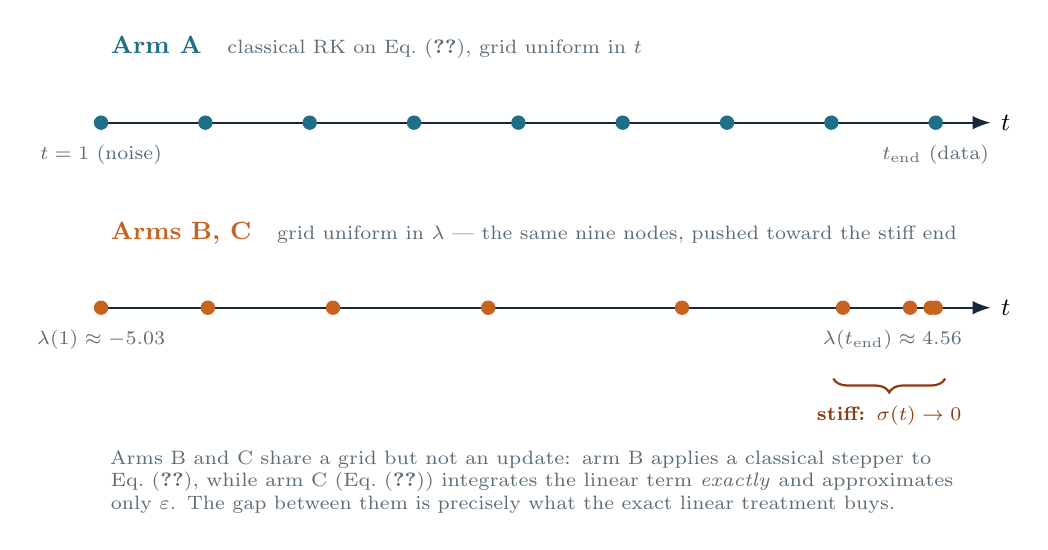
\begin{tikzpicture}[font=\small,>=Latex]

% ---------- arm A: uniform in t ----------
\begin{scope}[yshift=0cm]
  \node[anchor=west] at (0,.95)
    {\textcolor{armA}{\bfseries Arm A}\quad
     \textcolor{soft}{\scriptsize classical RK on Eq.~\eqref{eq:armA}, grid uniform in $t$}};
  \draw[->,thick,ink] (0,0) -- (11.3,0) node[right,black]{$t$};
  \foreach \x in {0,1.325,2.65,3.975,5.3,6.625,7.95,9.275,10.6}
    \fill[armA] (\x,0) circle (2.6pt);
  \node[below,soft,font=\scriptsize] at (0,-.16) {$t=1$ (noise)};
  \node[below,soft,font=\scriptsize] at (10.6,-.16) {$t_{\text{end}}$ (data)};
\end{scope}

% ---------- arms B and C: uniform in lambda, drawn on the same t axis ----------
\begin{scope}[yshift=-2.35cm]
  \node[anchor=west] at (0,.95)
    {\textcolor{armB}{\bfseries Arms B, C}\quad
     \textcolor{soft}{\scriptsize grid uniform in $\lam$ --- the same nine nodes,
     pushed toward the stiff end}};
  \draw[->,thick,ink] (0,0) -- (11.3,0) node[right,black]{$t$};
  % t(lambda_i) for nine nodes uniform in lambda, from src/schedule.py
  \foreach \x in {0,1.357,2.946,4.917,7.378,9.423,10.274,10.536,10.6}
    \fill[armB] (\x,0) circle (2.6pt);
  \node[below,soft,font=\scriptsize] at (0,-.16) {$\lam(1)\approx-5.03$};
  \node[below,soft,font=\scriptsize] at (10.05,-.16) {$\lam(t_{\text{end}})\approx4.56$};
\end{scope}

% ---------- the stiff region ----------
\draw[decorate,decoration={brace,amplitude=5pt,mirror},warn,thick]
      (9.30,-3.25) -- (10.72,-3.25)
      node[midway,below=6pt,warn,font=\scriptsize\bfseries]{stiff: $\sigma(t)\to0$};

\node[anchor=north west,soft,font=\scriptsize,text width=11.2cm] at (0,-4.05)
 {Arms B and C share a grid but not an update: arm B applies a classical stepper
  to Eq.~\eqref{eq:armB}, while arm C (Eq.~\eqref{eq:armC}) integrates the linear
  term \emph{exactly} and approximates only $\eps$. The gap between them is
  precisely what the exact linear treatment buys.};
\end{tikzpicture}
\caption{The three arms. All integrate one trajectory; they differ in the time
variable that is discretised uniformly and in how much of the right-hand side is
approximated. A uniform-$\lam$ grid automatically clusters nodes where the
problem stiffens.}
\label{fig:arms}
\end{figure}

% =====================================================================
\section{Experimental design}
% =====================================================================

\subsection{Three tiers}

To measure error one needs the right answer, which for a real generated image
does not exist. We therefore build deliberately simplified problems whose exact
solution is available, and step up in realism (Figure~\ref{fig:tiers}).

\paragraph{Tier 1 --- anisotropic Gaussian.}
For data $\sim\mathcal N(0,\operatorname{diag}(s))$ the ODE decouples into $d$
independent scalar linear ODEs. Both the score and the entire trajectory are
closed form:
\begin{equation}
\eps^{*}(x,t)_j = \frac{\sigma(t)\,x_j}{v_j(t)},\qquad
x_j(t) = x_j(T)\sqrt{\frac{v_j(t)}{v_j(T)}},\qquad
v_j(t) = \alpha(t)^2 s_j + \sigma(t)^2 .
\end{equation}
The stiffness knob is the condition number $\kappa = s_{\max}/s_{\min}$, which
we sweep over five decades. Because the linear case decouples, dimension changes
nothing --- we sweep $\kappa$, not $d$.

\paragraph{Tier 2 --- Gaussian/point mixture.}
Replacing the single Gaussian by a weighted point cloud $\mu_1,\dots,\mu_K$
keeps the score closed form but makes it genuinely nonlinear in $x$: the
posterior mean becomes a softmax over modes,
\begin{equation}
r_k \propto w_k \exp\!\left(-\frac{\lVert x-\alpha(t)\mu_k\rVert^2}{2\sigma(t)^2}\right),
\quad \hat x_0 = \sum_k r_k \mu_k,
\quad \eps^{*}(x,t) = \frac{x-\alpha(t)\hat x_0}{\sigma(t)} .
\end{equation}
We place $K=8$ modes on a Swiss-roll curve. There is no algebraic trajectory, so
the reference is SciPy's \textsc{dop853} at \texttt{rtol}~$=10^{-13}$,
\texttt{atol}~$=10^{-14}$, verified converged by recomputation at $10^{-11}$
(agreement $6.9\times10^{-13}$, far below every measured error). The
responsibilities are computed with \texttt{logsumexp}; a naive
$\exp$-then-normalise overflows long before the ratios cease to be well defined.

\paragraph{Tier 3 --- the real network.}
\texttt{google/ddpm-cifar10-32}, $d = 3072$, on a Kaggle T4. The reference is a
201-\NFE\ DPM-Solver-3 run of the \emph{same} checkpoint from the \emph{same}
$x_T$, so what is measured remains discretisation error rather than model error.

\begin{figure}[t]
\centering
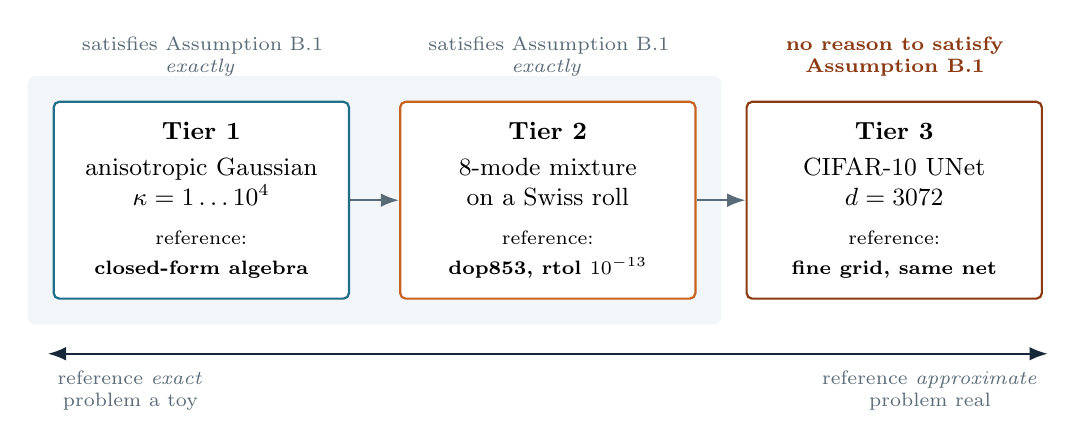
\begin{tikzpicture}[font=\small,>=Latex,
  tier/.style={draw=ink,rounded corners=2pt,minimum width=3.75cm,minimum height=2.5cm,
               align=center,inner sep=5pt,fill=white},
  lab/.style={font=\scriptsize,soft,align=center}]

\node[tier,draw=armA,thick] (t1) at (0,0)
  {\textbf{Tier 1}\\[2pt] anisotropic Gaussian\\ $\kappa = 1\dots10^{4}$\\[3pt]
   \scriptsize reference:\\ \scriptsize\textbf{closed-form algebra}};
\node[tier,draw=armB,thick] (t2) at (4.4,0)
  {\textbf{Tier 2}\\[2pt] 8-mode mixture\\ on a Swiss roll\\[3pt]
   \scriptsize reference:\\ \scriptsize\textbf{\textsc{dop853}, rtol $10^{-13}$}};
\node[tier,draw=warn,thick] (t3) at (8.8,0)
  {\textbf{Tier 3}\\[2pt] CIFAR-10 UNet\\ $d = 3072$\\[3pt]
   \scriptsize reference:\\ \scriptsize\textbf{fine grid, same net}};

\draw[->,thick,soft] (t1) -- (t2);
\draw[->,thick,soft] (t2) -- (t3);

\draw[<->,thick,ink] (-1.95,-1.95) -- (10.75,-1.95);
\node[lab,anchor=north west] at (-1.95,-2.05) {reference \emph{exact}\\ problem a toy};
\node[lab,anchor=north east] at (10.75,-2.05) {reference \emph{approximate}\\ problem real};

\node[lab,anchor=south,text width=3.6cm] at (0,1.45)
  {satisfies Assumption B.1\\ \emph{exactly}};
\node[lab,anchor=south,text width=3.6cm] at (4.4,1.45)
  {satisfies Assumption B.1\\ \emph{exactly}};
\node[anchor=south,text width=3.6cm,font=\scriptsize\bfseries,warn,align=center] at (8.8,1.45)
  {no reason to satisfy\\ Assumption B.1};

\begin{scope}[on background layer]
  \node[fit=(t1)(t2),rounded corners=3pt,fill=armA!6,inner sep=9pt] {};
\end{scope}
\end{tikzpicture}
\caption{The tier ladder. Moving right trades exactness of the reference for
realism of the problem. The shaded pair have analytic scores, hence continuous
derivatives to all orders --- they satisfy the order theorem's smoothness
hypothesis by construction. Tier 3 does not, which is what makes the comparison
a test rather than a demonstration.}
\label{fig:tiers}
\end{figure}

\subsection{Conventions}

Three decisions were fixed before any measurement and never revisited.
\textbf{Float64 everywhere} on Tiers 1--2: a float32 error floor near $10^{-7}$
would destroy the order fits. \textbf{Every run seeded.} \textbf{One results
schema} --- every experiment appends a row
\texttt{(tier, testbed, arm, solver, order, kappa, h, nfe, err\_l2, diverged,
seed)} to a CSV, so all tables concatenate without adapters.

Two accounting rules matter throughout. \NFE\ is \emph{not} step count: RK4
spends four network calls per step, DPM-Solver-$k$ spends $k$, and AB2 spends one
after startup. Every cross-arm comparison uses \emph{measured} \NFE, obtained
from a call counter wrapped around the right-hand side rather than assumed from a
formula. And order is defined in $h$, not \NFE; since arms measure $h$ in
different units, $h$ is used only \emph{within} an arm.

\subsection{Fitting an order}

A real convergence curve has three regions: pre-asymptotic at large $h$ where
theory does not yet apply, a straight middle, and a round-off floor at small $h$.
Fitting one line through all points averages across regimes and reports the wrong
number. We instead search every contiguous log--log subwindow and keep the one
that is both straight and wide, and we report the fit window and $R^2$ beside
every slope. This procedure is not infallible --- \S\ref{sec:tier3} documents a
case where it must be told about the floor explicitly.

\subsection{Validation: Gate G1}

Section 4.1 of the paper proves DDIM and DPM-Solver-1 are algebraically the same
update. Two independent implementations must therefore agree to machine
precision. Ours agree to $5.5\times10^{-16}$ against a $10^{-14}$ bar, and
DPM-Solver-1 measures at order $0.99$. Everything downstream was gated on this.
Separately, the Tier-1 closed-form trajectory satisfies the ODE to $\sim10^{-11}$
by finite difference and matches an independent \textsc{dop853} integration to
$10^{-12}$; our schedule agrees with the vendored
\texttt{NoiseScheduleVP('linear')} to $10^{-11}$, so all three arms provably
share one schedule.

We use the authors' own solver file, unmodified and pinned to a commit, driven by
an analytic oracle. This tests the \emph{published implementation} with zero
model error rather than a reimplementation of it.

% =====================================================================
\section{Results on the analytic tiers}
% =====================================================================

\subsection{Order}

Table~\ref{tab:order12} gives the measured slopes. Every solver in every arm
attains its theoretical order: the worst deviation is $0.094$ on Tier 1 and
$0.084$ on Tier 2, with mean $R^2$ of $0.99992$ and $0.99996$. Introducing
genuine curvature (Tier 2) shifts no slope by more than $0.059$.

This is the control experiment. Both tiers have analytic scores, so Assumption
B.1 holds exactly, and the order theorem's conclusion holds exactly with it.

\begin{table}[t]
\centering
\caption{Measured convergence order on the two exact-score testbeds. Slopes are
log--log fits of $\lVert x_N - x_{\text{ref}}\rVert_2$ against $h$ over the
automatically selected asymptotic window.}
\label{tab:order12}
\small
\begin{tabular}{llcccc}
\toprule
Arm & Solver & Theory $p$ & Tier 1 & Tier 2 & $|\Delta|$ max \\
\midrule
A & euler     & 1 & 1.012 & 1.012 & 0.012 \\
A & midpoint  & 2 & 2.028 & 2.031 & 0.031 \\
A & heun3     & 3 & 3.014 & 2.999 & 0.014 \\
A & rk4       & 4 & 3.938 & 3.997 & 0.062 \\
A & ab2       & 2 & 2.033 & 1.988 & 0.033 \\
\midrule
B & euler     & 1 & 1.023 & 1.023 & 0.023 \\
B & midpoint  & 2 & 2.057 & 2.055 & 0.057 \\
B & heun3     & 3 & 3.015 & 3.024 & 0.024 \\
B & rk4       & 4 & 3.921 & 3.965 & 0.079 \\
B & ab2       & 2 & 1.935 & 1.975 & 0.065 \\
\midrule
C & ddim      & 1 & 0.994 & 0.996 & 0.006 \\
C & dpm1      & 1 & 0.994 & 0.996 & 0.006 \\
C & dpm2      & 2 & 2.028 & 2.018 & 0.028 \\
C & dpm3      & 3 & 3.094 & 3.084 & 0.094 \\
\bottomrule
\end{tabular}
\end{table}

\subsection{Stability: a claim that does not reproduce}

Section 4.2 of the paper asserts that explicit methods on this semi-linear ODE
destabilise at large steps near $t\!\to\!0$. We measured it directly, bisecting
on step count for the coarsest grid that remains bounded, across
$\kappa\in\{1,10,10^2,10^3,10^4\}$ and all five steppers in both arms.

\textbf{The stability map is exactly flat.} Arm A reports the coarsest grid tried
($h \approx 0.4995$) as already stable for every $\kappa$ and every stepper;
arm B likewise at $h \approx 4.7913$. The variation across five decades of
$\kappa$ is identically zero. Stress-testing to $\kappa = 10^{8}$ and
$t_{\text{end}} = 10^{-6}$ changed nothing.

This is not a bug --- the bisection is verified separately against a synthetic
linear ODE with a closed-form instability threshold. It is structural. On a
uniform-$t$ grid the node nearest the boundary sits at $t_{\text{end}}+h$, and the
exact stability product $h\cdot J(t_{\text{end}}+h)$, with $J$ the local
Jacobian, never exceeds ${\approx}\,0.9$ for any $h$ or $\kappa$ --- comfortably
under explicit Euler's threshold of 2 --- because $\sigma(t)^2 \sim \beta_0 t$
near the boundary makes the growing local stiffness and the grid's shrinking
distance to $t_{\text{end}}$ very nearly cancel.

We therefore \emph{narrow} rather than confirm the paper's \S4.2 claim: it does
not manifest on a linear, decoupled problem under this metric. It may still hold
under a different stability definition or on a problem where the cancellation has
no reason to occur.

\subsection{The crossover}

Table 6 of the base paper reports, without explanation, that DPM-Solver-3 is
dramatically \emph{worse} than DPM-Solver-1 at ${\sim}10$ \NFE\ on CIFAR-10
(FID 18.37 versus 11.83 at $\epsilon = 10^{-3}$). This is textbook
pre-asymptotic behaviour: at large $h$ the cubic Taylor correction is not yet
valid and actively hurts. With exact answers and a continuously sweepable $h$ we
can locate the crossing precisely, comparing the two orders at \emph{matched
$h$} (a shared macro-step count, so both share the step size and differ only in
\NFE\ cost).

\begin{table}[h]
\centering
\caption{Crossover step size $h^\star$ and the corresponding DPM-Solver-3 budget,
at $t_{\text{end}} = 10^{-3}$ (the paper's own $\epsilon$).}
\label{tab:crossover}
\small
\begin{tabular}{llcc}
\toprule
Testbed & $\kappa$ & $h^\star$ & $\NFE_3^\star$ \\
\midrule
Tier 1, Gaussian & $1$      & 6.497 & 4.43 \\
Tier 1, Gaussian & $10$     & 6.157 & 4.67 \\
Tier 1, Gaussian & $10^{2}$ & 5.795 & 4.96 \\
Tier 1, Gaussian & $10^{3}$ & 6.131 & 4.69 \\
Tier 1, Gaussian & $10^{4}$ & 6.228 & 4.62 \\
\midrule
Tier 2, \texttt{mog8} & --- & 3.219 & 8.93 \\
\bottomrule
\end{tabular}
\end{table}

The crossover is real and reproducible, and $\NFE_3^\star$ is \emph{flat across
five decades of stiffness} --- echoing the stability finding. Curvature, not
stiffness, moves it: Tier 2 crosses at $8.93$, roughly double Tier 1 and much
closer to the paper's observed 10--12. Neither analytic tier reaches that value,
and both still have an exact score. The residual gap is therefore attributable to
the two ingredients they lack --- network approximation error and much higher
intrinsic dimension --- which is precisely what Tier 3 supplies.

% =====================================================================
\section{Tier 3: the order theorem meets a real network}
\label{sec:tier3}
% =====================================================================

\subsection{One schedule, read off the checkpoint}

The CIFAR-10 checkpoint is a \emph{discrete-time} DDPM: 1000 $\beta$ values, with
$\log\alpha$ linearly interpolated between tabulated times. That is the same
VP-linear schedule discretised, and it is \emph{not} interchangeable with the
continuous form --- we measure $\max|\Delta\lam| = 4.74\times10^{-2}$ and a
$5.0\%$ discrepancy in $f$. Using continuous coefficients for arms A and B would
place a systematic $5\%$ error beneath every Tier-3 curve.

We therefore derive all three arms from the checkpoint's own schedule. Arm B
needs only $\hat\sigma(\lam)$ --- which follows from $\lam = \log\alpha-\log\sigma$
and $\alpha^2+\sigma^2=1$ alone, hence is exact for any variance-preserving
schedule --- and $t(\lam)$. Arm A needs $f$ and $g^2$, and here one identity does
all the work. Differentiating $\sigma^2 = 1-\alpha^2$ gives
$\sigma' = -\alpha^2 f/\sigma$, so
\begin{equation}
\lam' = f - \frac{\sigma'}{\sigma} = f\left(1+\frac{\alpha^2}{\sigma^2}\right) = \frac{f}{\sigma^2},
\qquad\text{hence}\qquad
\boxed{\;f = \sigma^2\lam',\qquad g^2 = -2\sigma^2\lam' = -2f.\;}
\label{eq:vpid}
\end{equation}
Taking \emph{both} coefficients from a single central difference of $\lam$ makes
$f/\lam' \equiv \sigma^2$ hold to $1.1\times10^{-16}$ rather than approximately
--- and that identity is exactly what makes \eqref{eq:armA} and \eqref{eq:armB}
the same ODE. Arms A and B therefore agree by construction; we verify it end to
end, integrating both at four resolutions and watching the gap fall from
$2.5\times10^{-4}$ to $3.9\times10^{-7}$.

\subsection{Order collapses in proportion to the order claimed}

Table~\ref{tab:order3} is the central result of this report.

\begin{table}[t]
\centering
\caption{Measured order against a real network, beside the exact-score tiers.
``Floor-excl.'' refits after discarding sweep points within $3\times$ the
measured reference floor, as the base paper's own guidance requires (``do not
fit slopes through the flat part''); ``drop'' is how many of the eight points
that removes. Only the three curves that actually reach the floor are affected.
Produced by \texttt{notebooks/10\_report.ipynb} into
\texttt{results/master\_order\_table.csv}.}
\label{tab:order3}
\small
\begin{tabular}{llccccrc}
\toprule
Arm & Solver & Theory $p$ & Tier 1 & Tier 2 & Tier 3 & Floor-excl. & drop \\
\midrule
A & euler    & 1 & 1.012 & 1.012 & \textbf{0.842} & 0.842 & 0 \\
A & midpoint & 2 & 2.028 & 2.031 & \textbf{1.525} & 1.500 & 1 \\
A & rk4      & 4 & 3.938 & 3.997 & \textbf{1.210} & 1.210 & 0 \\
\midrule
B & euler    & 1 & 1.023 & 1.023 & \textbf{0.746} & 0.746 & 0 \\
B & midpoint & 2 & 2.057 & 2.055 & \textbf{1.603} & 1.603 & 0 \\
B & rk4      & 4 & 3.921 & 3.965 & \textbf{2.231} & $1.099^{\dagger}$ & 2 \\
\midrule
C & dpm1     & 1 & 0.994 & 0.996 & \textbf{0.813} & 0.813 & 0 \\
C & dpm2     & 2 & 2.028 & 2.018 & \textbf{2.191} & 2.244 & 1 \\
C & dpm3     & 3 & 3.094 & 3.084 & \textbf{2.473} & \textbf{2.995} & 1 \\
\bottomrule
\end{tabular}

\vspace{2pt}
{\footnotesize $^{\dagger}$ \texttt{B/rk4} loses two of eight points to the
floor, leaving six that lie mostly in its pre-asymptotic region. Neither number
should be trusted for that row: at these budgets it has no clean asymptotic
window at all, which is itself the finding.}
\end{table}

The worst deviation from theory goes $0.094$ (Tier 1) $\to$ $0.084$ (Tier 2)
$\to$ $2.790$ (Tier 3): a factor of thirty-three. Eight of nine fits sit more
than $0.15$ below theory.

The \emph{structure} of the loss is what makes this a test of Assumption B.1
rather than a generic complaint about neural networks. The assumption requires
the model's derivatives with respect to $\lam$ to exist and be continuous up to
order $k+1$. A $p$th-order scheme leans on derivatives up to order $p$; if those
derivatives are not there, the higher-order scheme has more to lose. That is
exactly the observed pattern:
\begin{center}
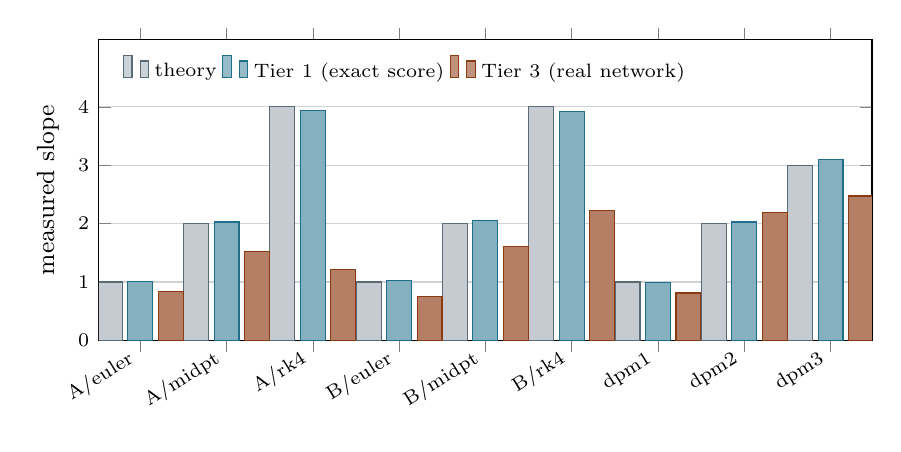
\begin{tikzpicture}
\begin{axis}[
  width=11.4cm, height=5.4cm,
  ybar, bar width=9pt,
  ymin=0, ymax=5.15,
  ylabel={measured slope}, ylabel style={font=\small},
  symbolic x coords={A/euler,A/midpt,A/rk4,B/euler,B/midpt,B/rk4,dpm1,dpm2,dpm3},
  xtick=data, x tick label style={font=\scriptsize,rotate=32,anchor=east},
  ytick={0,1,2,3,4}, tick label style={font=\scriptsize},
  legend style={font=\scriptsize,at={(0.02,0.97)},anchor=north west,draw=none,fill=white,fill opacity=.85,text opacity=1},
  legend columns=3,
  major grid style={soft!30}, ymajorgrids,
  enlarge x limits=0.06,
]
\addplot[fill=soft!35,draw=soft] coordinates
 {(A/euler,1)(A/midpt,2)(A/rk4,4)(B/euler,1)(B/midpt,2)(B/rk4,4)(dpm1,1)(dpm2,2)(dpm3,3)};
\addplot[fill=armA!55,draw=armA] coordinates
 {(A/euler,1.012)(A/midpt,2.028)(A/rk4,3.938)(B/euler,1.023)(B/midpt,2.057)(B/rk4,3.921)(dpm1,0.994)(dpm2,2.028)(dpm3,3.094)};
\addplot[fill=warn!65,draw=warn] coordinates
 {(A/euler,0.842)(A/midpt,1.525)(A/rk4,1.210)(B/euler,0.746)(B/midpt,1.603)(B/rk4,2.231)(dpm1,0.813)(dpm2,2.191)(dpm3,2.473)};
\legend{theory, Tier 1 (exact score), Tier 3 (real network)}
\end{axis}
\end{tikzpicture}
\end{center}

RK4 in arm A sheds $2.79$ of its four claimed orders; explicit Euler sheds
$0.16$ of its one. The methods that assumed the most smoothness lost the most
when it was absent. (The bars show the primary Tier-3 column; \texttt{dpm3}
reads $2.995$ once its one floor-bound point is excluded, as discussed below.)

Two qualifications keep this honest. First, \texttt{dpm3} is the striking
exception once the floor is handled properly: discarding the single point that
reaches it restores $2.995$, essentially its textbook order. DPM-Solver-3 is the
one scheme here that \emph{holds} its order against a real network --- a result
favourable to the base paper, and one we would have missed by trusting the
automatic window search, which prefers a wider window and will fit straight
through a flat tail unless told where the floor is. Note the asymmetry that makes
this a real effect rather than a fitting artefact: the curves \emph{far} from the
floor (\texttt{A/rk4} at $12\times$ it, \texttt{B/euler} at $42\times$) lose
nothing to the exclusion and still measure far below theory. The order collapse
and the floor are independent phenomena. Second, the Tier-3 sweep spans 10--120 \NFE, which for
the higher-order arm-A/B methods is partly pre-asymptotic by construction; that
band is the practically interesting one, but it is not a clean asymptotic
measurement, and the low slopes should be read as ``what you actually get at
practitioner budgets'', not as a refutation of the theorem's algebra.

\subsection{The reparameterisation finally earns its keep}

On the analytic tiers arms A and B are nearly indistinguishable --- their slopes
differ by hundredths. Against a real network they separate sharply. Arm A's RK4
measures $1.21$ and bottoms out at an error of $4.57$; arm B's measures $2.23$
and reaches $0.43$ --- \textbf{ten times better at the same budget}
(Figure~\ref{fig:t3nfe}). The $\lam$-reparameterisation, worth almost nothing
when the score is exact, is worth an order of magnitude when it is not. This is
the A-versus-B comparison the three-arm design exists to make, and it only
becomes visible at Tier 3.

\begin{figure}[t]
\centering
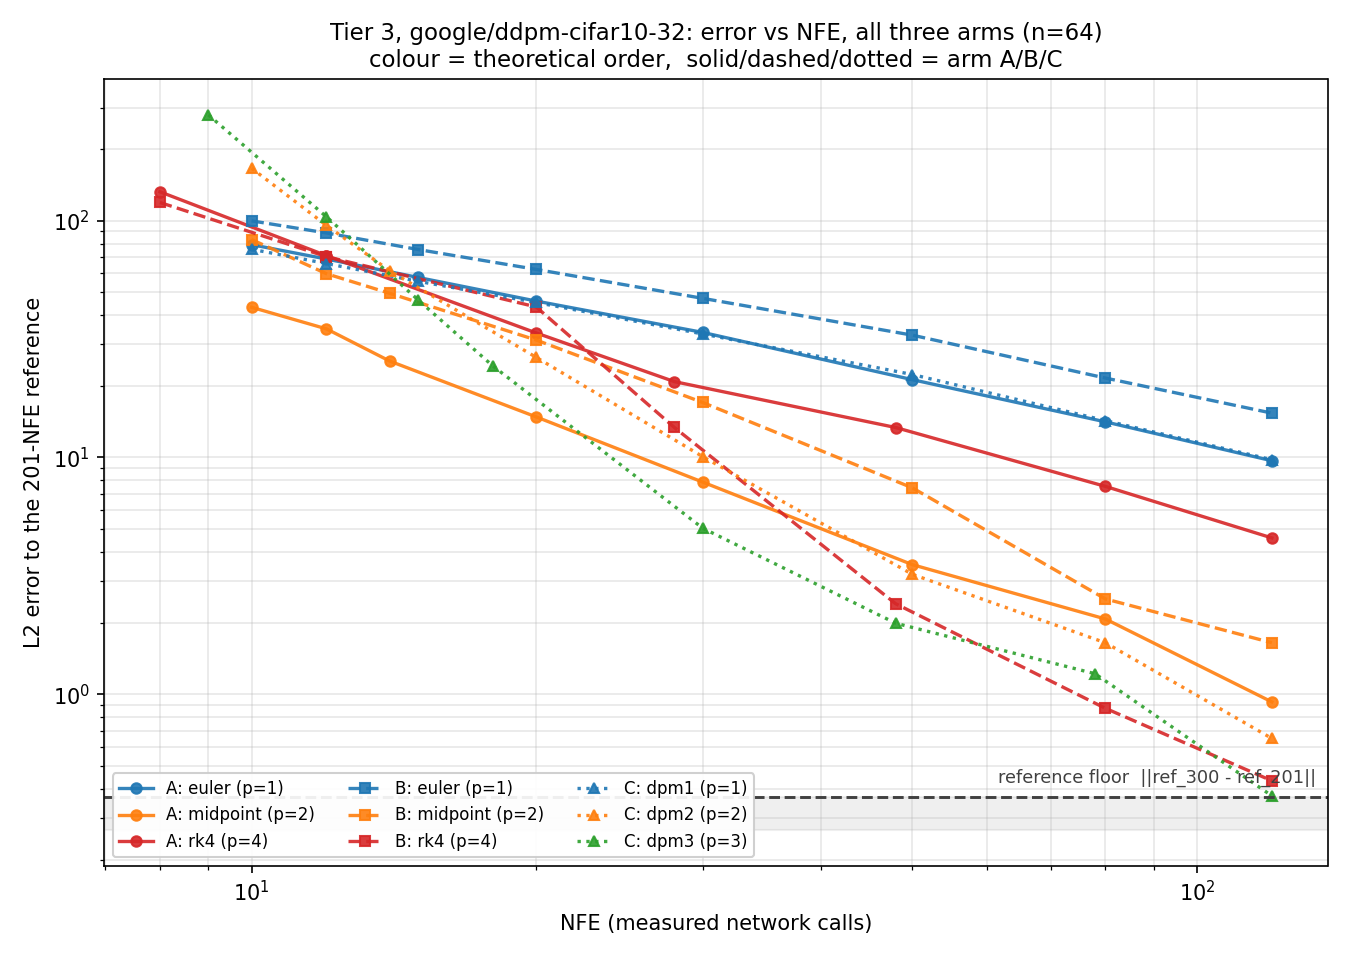
\includegraphics[width=0.94\textwidth]{09_tier3_error_vs_nfe.png}
\caption{Tier 3: error against measured \NFE\ for all nine solver/arm
combinations. Colour encodes theoretical order, line style encodes arm. The
dashed horizontal line is the reference's own uncertainty
$\lVert x_{300}-x_{201}\rVert$; nothing below it is a measurement of
discretisation error. Note the separation between solid and dashed red
(arm A versus arm B RK4).}
\label{fig:t3nfe}
\end{figure}

\subsection{The three-way error decomposition}

Total Tier-3 error has three components, not one, and each is measurable without
knowing the true score (Figure~\ref{fig:decomp}).

\begin{center}
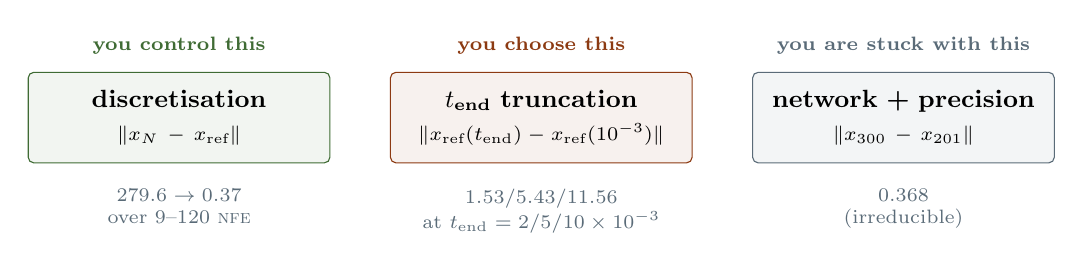
\begin{tikzpicture}[font=\small,>=Latex,
  box/.style={draw,rounded corners=2pt,minimum height=1.15cm,text width=3.55cm,
              align=center,inner sep=4pt,font=\small}]
\node[box,draw=armC,fill=armC!7] (d) at (0,0)
  {\textbf{discretisation}\\[1pt]\scriptsize $\lVert x_N - x_{\text{ref}}\rVert$};
\node[box,draw=warn,fill=warn!7] (t) at (4.6,0)
  {\textbf{$t_{\text{end}}$ truncation}\\[1pt]\scriptsize $\lVert x_{\text{ref}}(t_{\text{end}}) - x_{\text{ref}}(10^{-3})\rVert$};
\node[box,draw=soft,fill=soft!7] (n) at (9.2,0)
  {\textbf{network + precision}\\[1pt]\scriptsize $\lVert x_{300} - x_{201}\rVert$};

\node[below=2mm of d,font=\scriptsize,soft,align=center] {$279.6 \to 0.37$\\ over 9--120 \NFE};
\node[below=2mm of t,font=\scriptsize,soft,align=center] {$1.53 / 5.43 / 11.56$\\ at $t_{\text{end}}=2/5/10\times10^{-3}$};
\node[below=2mm of n,font=\scriptsize,soft,align=center] {$0.368$\\ (irreducible)};

\node[above=1mm of d,font=\scriptsize\bfseries,armC] {you control this};
\node[above=1mm of t,font=\scriptsize\bfseries,warn] {you choose this};
\node[above=1mm of n,font=\scriptsize\bfseries,soft] {you are stuck with this};
\end{tikzpicture}
\end{center}

The floor of $0.368$ total is $4.6\times10^{-2}$ per sample against
$\lVert x\rVert \approx \sqrt{3072} \approx 55$, i.e.\ ${\approx}\,8\times10^{-4}$
relative --- matching the ${\sim}10^{-3}$ float32 floor the base paper's
practitioners would predict, here measured rather than assumed.

The instructive comparison is between the second and first columns. Truncating at
$t_{\text{end}} = 2\times10^{-3}$ instead of $10^{-3}$ moves the endpoint by
$1.53$ --- more than DPM-Solver-3's entire discretisation error at 78 \NFE\
($1.22$). Past that budget, refining the grid buys accuracy the truncation
choice immediately throws away. This is the mechanism behind the base paper's own
Table 4, where FID \emph{worsens} from 4.39 at 15 \NFE\ to 5.52 at 20: the
discretisation term has dropped below the truncation term, and the extra network
calls are being spent on the wrong error.

\begin{figure}[t]
\centering
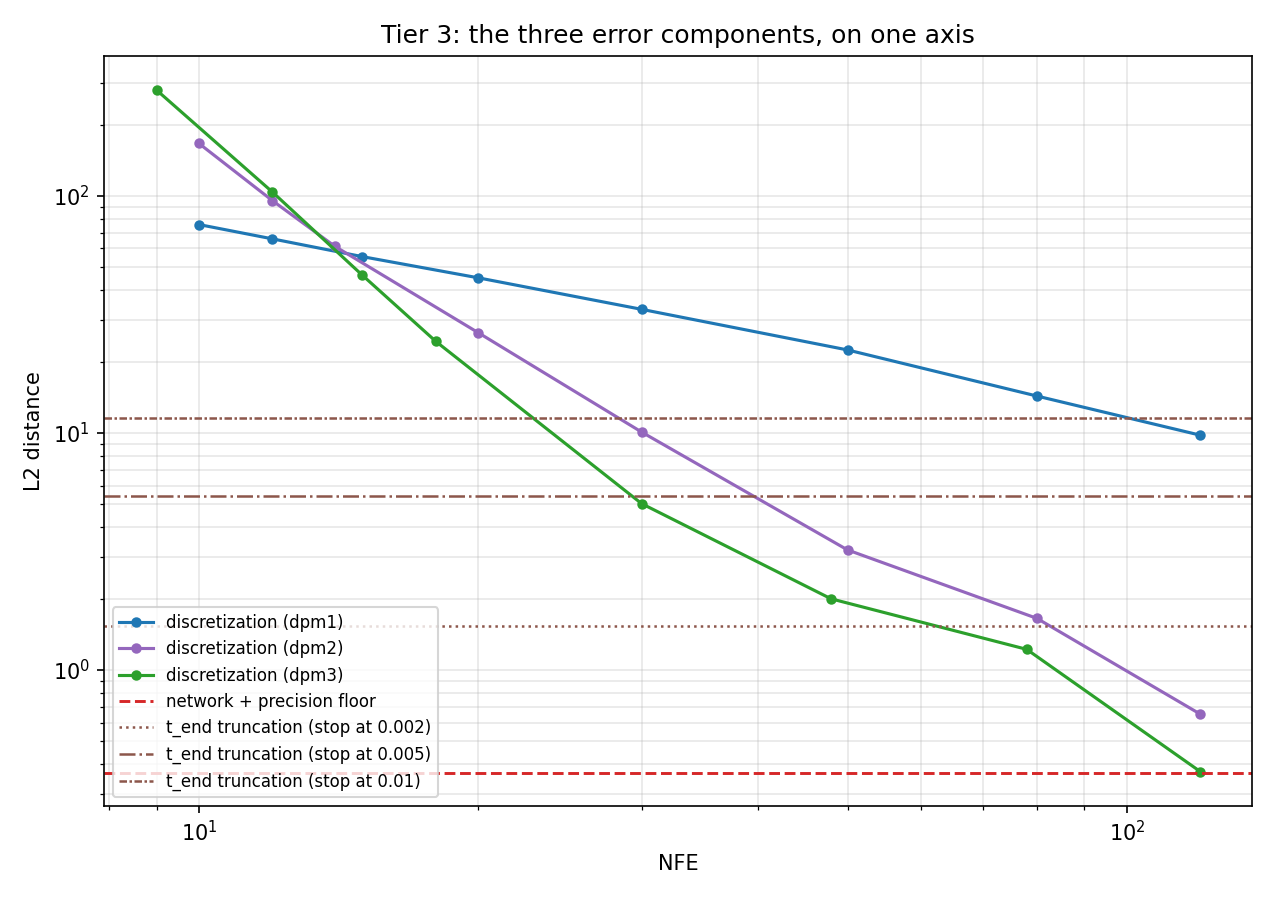
\includegraphics[width=0.92\textwidth]{09_tier3_decomposition.png}
\caption{The three components on one axis. Where a discretisation curve crosses a
horizontal line, that component ceases to dominate and further \NFE\ stops buying
end-to-end accuracy.}
\label{fig:decomp}
\end{figure}

% =====================================================================
\section{The ledger}
% =====================================================================

We wrote six predictions down before measuring. Reporting the misses is more
useful than reporting only the hits.

\begin{table}[h]
\centering
\caption{Predictions and outcomes. Every verdict is computed from the results
CSVs by \texttt{notebooks/10\_report.ipynb}, not asserted by hand.}
\label{tab:ledger}
\small
\begin{tabular}{@{}p{7.15cm}lp{5.95cm}@{}}
\toprule
Prediction & Verdict & Evidence \\
\midrule
Tiers 1--2 slopes match theory within $\pm0.15$ & \textbf{confirmed} &
worst $|\Delta| = 0.094$ over 28 fits; mean $R^2 = 0.99994$ \\[3pt]
Arm A degrades as $\kappa$ grows; arms B/C do not & \textbf{refuted} &
$h_{\max}$ flat for every arm and stepper; variation across $\kappa\in[1,10^4]$
is exactly $0$ \\[3pt]
Euler-$\lam$ and DPM-Solver-1 are both first order but not identical &
\textbf{confirmed} & slopes $1.02$ vs $0.99$; errors differ by $1.4\times$ at
matched \NFE \\[3pt]
RK4 wins per step, loses per \NFE, to DPM-Solver-3 & \textbf{narrowed} &
holds on Tier 3 for \NFE\ 16--120; fails on Tiers 1--2, whose sweeps sit deep in
the asymptotic regime where $h^4$ dominates \\[3pt]
Tier-3 slopes come out lower than theory and flatten early & \textbf{confirmed} &
8 of 9 fits $>0.15$ below theory; worst gap $-2.79$ \\[3pt]
Arm B at low \NFE\ may be worse than arm A & \textbf{confirmed} &
observed on all three tiers at the coarsest shared budget \\
\bottomrule
\end{tabular}
\end{table}

\paragraph{Departures from the proposal.} The efficiency frontier is reported in
\NFE\ rather than wall-clock (the paper's Table 7 shows runtime is linear in \NFE\
and near-identical across solvers, so wall-clock adds nothing). Tier 1 sweeps
$\kappa$ at fixed $d$ rather than $d = 2\dots100$, because the linear case
decouples and dimension changes nothing. Tier 2 uses a point mixture rather than a
continuous Swiss roll, which has no closed-form score. The reference tolerance is
$10^{-13}$ rather than $10^{-14}$, which SciPy refuses. Adaptive RK45 was
\textbf{dropped}: step size is not a free variable for an adaptive method, so
neither ``order versus $h$'' nor ``maximum stable $h$'' is defined on it; AB2
restores the multistep row instead. FID was \textbf{dropped} at the
week-2 gate in favour of $L_2$-to-reference, which is both the primary metric and
the one consistent with this report's thesis. Added beyond the proposal: arm B,
Gate G1, the crossover study, and the three-way decomposition.

% =====================================================================
\section{Reproducibility}
% =====================================================================

The engine is plain Python under \texttt{src/}, unit-tested (108 tests), with no
GPU or plotting code. Notebooks import it, run the sweeps and write
\texttt{results/} and \texttt{figures/}. \texttt{run\_all.sh} reproduces every
figure and CSV from a clean clone; it skips only the Tier-3 notebook, which needs
a CUDA GPU and runs on Kaggle, and whose outputs are committed.

One implementation note worth recording: the same integrator and the same
right-hand side definition march all three tiers. \texttt{integrate} is
backend-agnostic (float64 NumPy on Tiers 1--2, float32 CUDA tensors on Tier 3)
and the probability-flow ODE is written once, parameterised by a schedule object.
The claim that arms A and B mean the same thing across tiers is therefore
structural rather than a matter of careful duplication.

% =====================================================================
\section{Conclusion}
% =====================================================================

Judged as a numerical method rather than an image generator, DPM-Solver holds up
well, and the interesting failures are elsewhere.

On testbeds with analytic scores, every solver we tested attains its textbook
order to within $0.1$ --- the order theorem is correct and our measurement
machinery is sound. Against a real network the picture changes: order collapses,
and it collapses in proportion to the order claimed, which is the signature of an
unsatisfied smoothness hypothesis rather than of numerical noise. DPM-Solver-3 is
the notable exception, retaining $2.995$ of its three orders once the measurement
floor is excluded properly.

Two of the paper's incidental claims came out differently than expected. Its
\S4.2 instability assertion does not reproduce on our stiff Tier-1 problem, for a
reason specific to the VP-linear schedule that we identify. And its unexplained
Table 6 anomaly --- order 3 losing to order 1 at ${\sim}10$ \NFE\ --- is real,
measurable, and driven by curvature rather than stiffness, though the analytic
tiers alone reach only $\NFE_3^\star \approx 8.9$ of the paper's 10--12.

The practical recommendation that falls out is narrower than ``use the highest
order available''. Higher order pays only where the integrand is smooth enough to
support it and only within a budget band that must be measured, not assumed; and
past roughly 78 \NFE\ on this checkpoint, the choice of $t_{\text{end}}$ costs
more than the discretisation does, so additional network calls are spent on the
wrong error entirely.

\vspace{4pt}
\noindent\rule{\linewidth}{0.4pt}\\[2pt]
{\footnotesize Base paper: C.~Lu, Y.~Zhou, F.~Bao, J.~Chen, C.~Li, J.~Zhu.
\emph{DPM-Solver: A Fast ODE Solver for Diffusion Probabilistic Model Sampling in
Around 10 Steps}. NeurIPS 2022, arXiv:2206.00927. Solver code MIT-licensed,
vendored unmodified at a pinned commit.}

\end{document}
